\begin{tikzpicture}
\begin{axis}[
    xlabel={$m$},
    ylabel={$\Phi(m)$},
    axis lines=middle,
    domain=-2:3,
    samples=100,
]
% nonlinear function
\addplot[blue, thick] {(x-1)^2 + 0.3*sin(deg(3*x))};

% quadratic approximation (schematic)
\addplot[red, dashed, domain=-1.5:1] {0.5*(x+0.5)^2 + 1};

% lines
\addplot[dotted] coordinates {(-1,0) (-1,5)};
\addplot[dotted] coordinates {(1,0) (1,3)};

\node at (axis cs:-1,4) {$m_i$};
\node at (axis cs:1,2.5) {$m_{i+1}$};

\end{axis}
\end{tikzpicture}

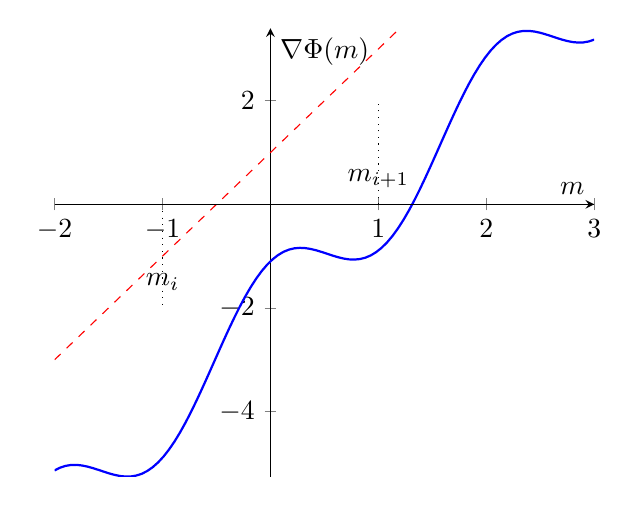
\begin{tikzpicture}
\begin{axis}[
    xlabel={$m$},
    ylabel={$\nabla \Phi(m)$},
    axis lines=middle,
    domain=-2:3,
    samples=100,
]
% gradient curve (schematic)
\addplot[blue, thick] {2*(x-1) + 0.9*cos(deg(3*x))};

% tangent line
\addplot[red, dashed, domain=-2:1.2] {-1 + 2*(x+1)};

% horizontal axis
\addplot[black] coordinates {(-2,0) (3,0)};

% verticals
\addplot[dotted] coordinates {(-1,0) (-1,-2)};
\addplot[dotted] coordinates {(1,0) (1,2)};

\node at (axis cs:-1,-1.5) {$m_i$};
\node at (axis cs:1,0.5) {$m_{i+1}$};

\end{axis}
\end{tikzpicture}